\documentclass[a4paper,11pt,titlepage]{jsarticle}
\usepackage[final]{graphicx}
\usepackage[dvipdfmx]{color}
\usepackage{listings, xcolor}
\usepackage{amsmath}
\usepackage{here}
\usepackage{tikz}

\lstset{
    basicstyle = {\ttfamily},
    frame = {tbrl},
    breaklines = true,
    numbers = left,
    showspaces = false,
    showstringspaces = false,
    showtabs = false,
    keywordstyle = \color{blue},
    commentstyle = {\color[HTML]{1AB91A}},
    identifierstyle = \color{black},
    stringstyle = \color{brown},
    captionpos = t
}

\title{画像処理レポート2}
\author{235738B 越後 玲輝}

\begin{document}

\maketitle
\tableofcontents
\newpage

\section{基本課題}

\subsection{1) 画像の表示}
\lstinputlisting[caption={課題1-1: 画像を表示}, label={lst:code1}]{code1.py}
\paragraph{実行結果}
\begin{figure}[H]
  \centering
  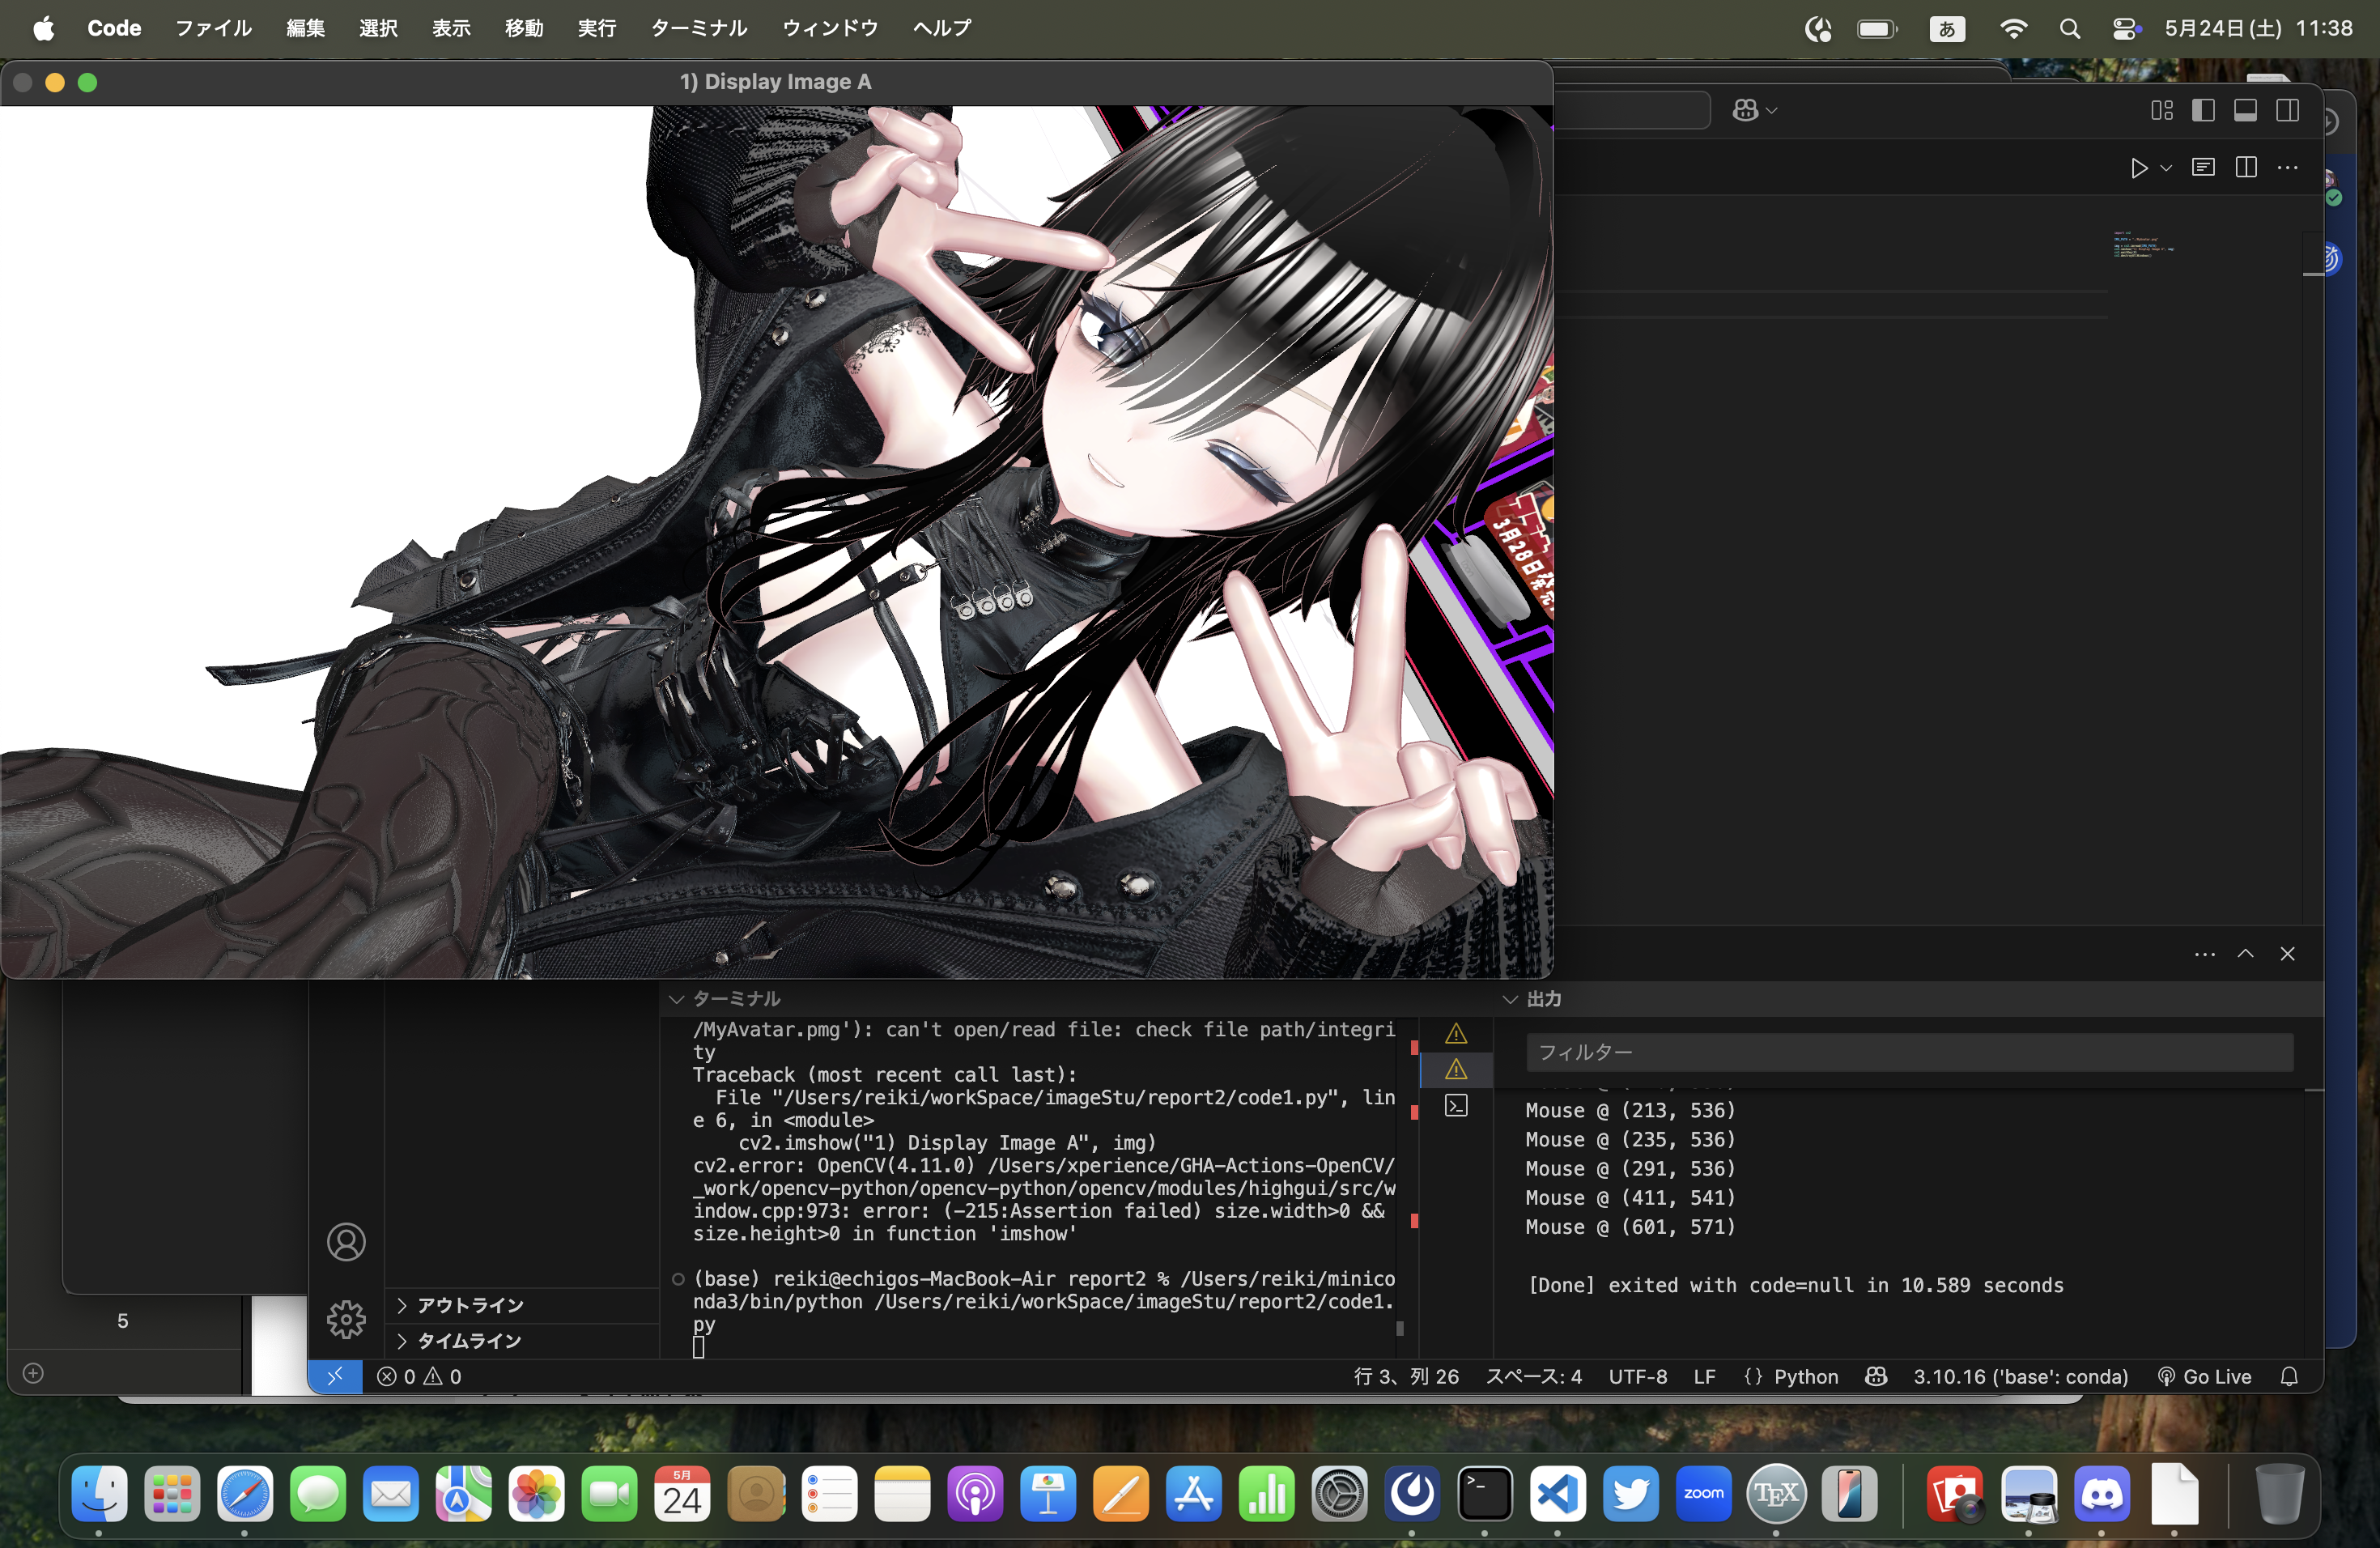
\includegraphics[width=0.8\textwidth]{code1-picture.png}
  \caption{課題1-1 実行結果}
\end{figure}

\subsection{2) マウスカーソル位置の出力}
\lstinputlisting[caption={課題1-2: マウスカーソルの位置を出力}, label={lst:code2}]{code2.py}
\paragraph{実行結果}
\begin{figure}[H]
  \centering
  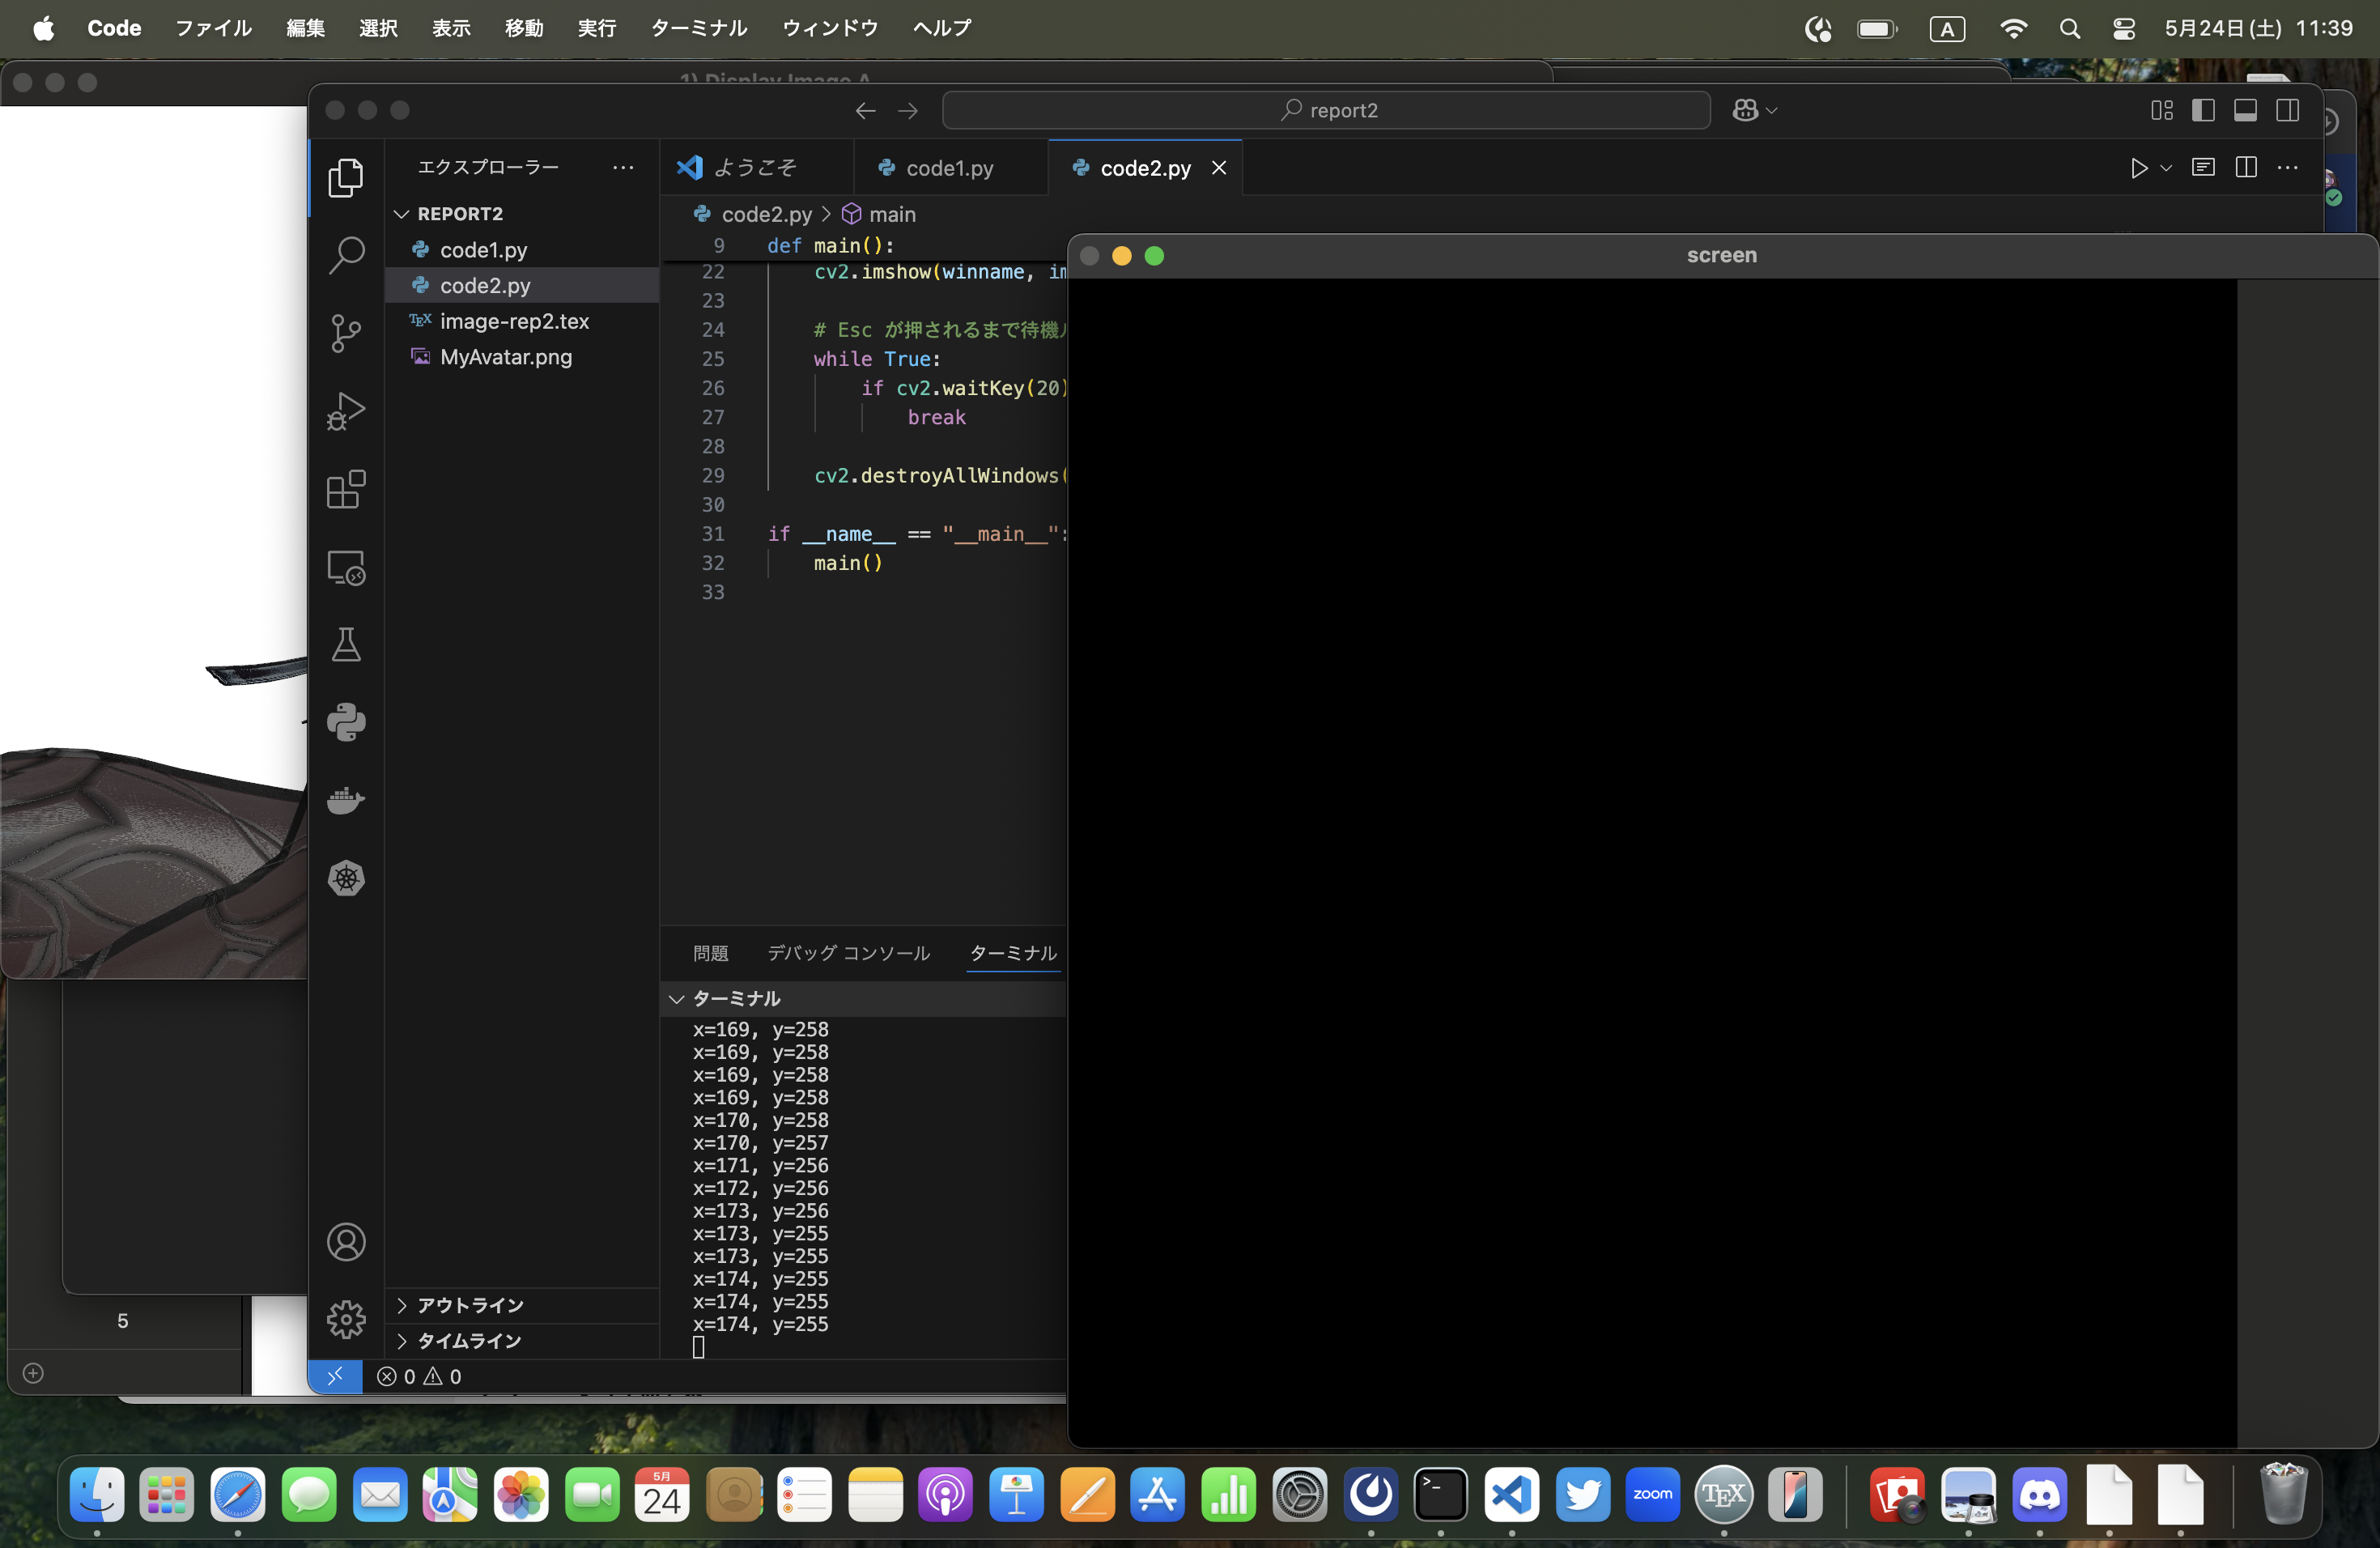
\includegraphics[width=0.8\textwidth]{code2-picture.png}
  \caption{課題1-2 実行結果}
\end{figure}

\subsection{3) 画素Pの位置を出力}
\lstinputlisting[caption={課題1-3: 指定画素の位置を出力}, label={lst:code3}]{code3.py}
\paragraph{実行結果}
\begin{figure}[H]
  \centering
  \includegraphics[width=0.8\textwidth]{code3-picture.png}
  \caption{課題1-3 実行結果}
\end{figure}

\subsection{4) 画素Pの画素値を出力}
\lstinputlisting[caption={課題1-4: 指定画素の画素値を出力}, label={lst:code4}]{code4.py}
\paragraph{実行結果}
\begin{figure}[H]
  \centering
  \includegraphics[width=0.8\textwidth]{code4-picture.png}
  \caption{課題1-4 実行結果}
\end{figure}

\subsection{5) 画像サイズの出力}
\lstinputlisting[caption={課題1-5: 画像サイズを出力}, label={lst:code5}]{code5.py}
\paragraph{実行結果}
\begin{figure}[H]
  \centering
  \includegraphics[width=0.8\textwidth]{code5-picture.png}
  \caption{課題1-5 実行結果}
\end{figure}

\subsection{6) 矩形領域の指定と描画}
\lstinputlisting[caption={課題1-6: 矩形領域を指定して描画}, label={lst:code6}]{code6.py}
\paragraph{実行結果}
\begin{figure}[H]
  \centering
  \includegraphics[width=0.8\textwidth]{code6-picture.png}
  \caption{課題1-6 実行結果}
\end{figure}

\section{発展課題}

\subsection{A7) 12枚の画像を6秒ずつ順番に表示}
\lstinputlisting[caption={課題A7: 6秒ずつ表示}, label={lst:code7}]{code7.py}
\begin{figure}[H]
  \centering
  \includegraphics[width=0.8\textwidth]{code7-picture1.png}
  \caption{課題A7 実行結果1}
\end{figure}
\begin{figure}[H]
  \centering
  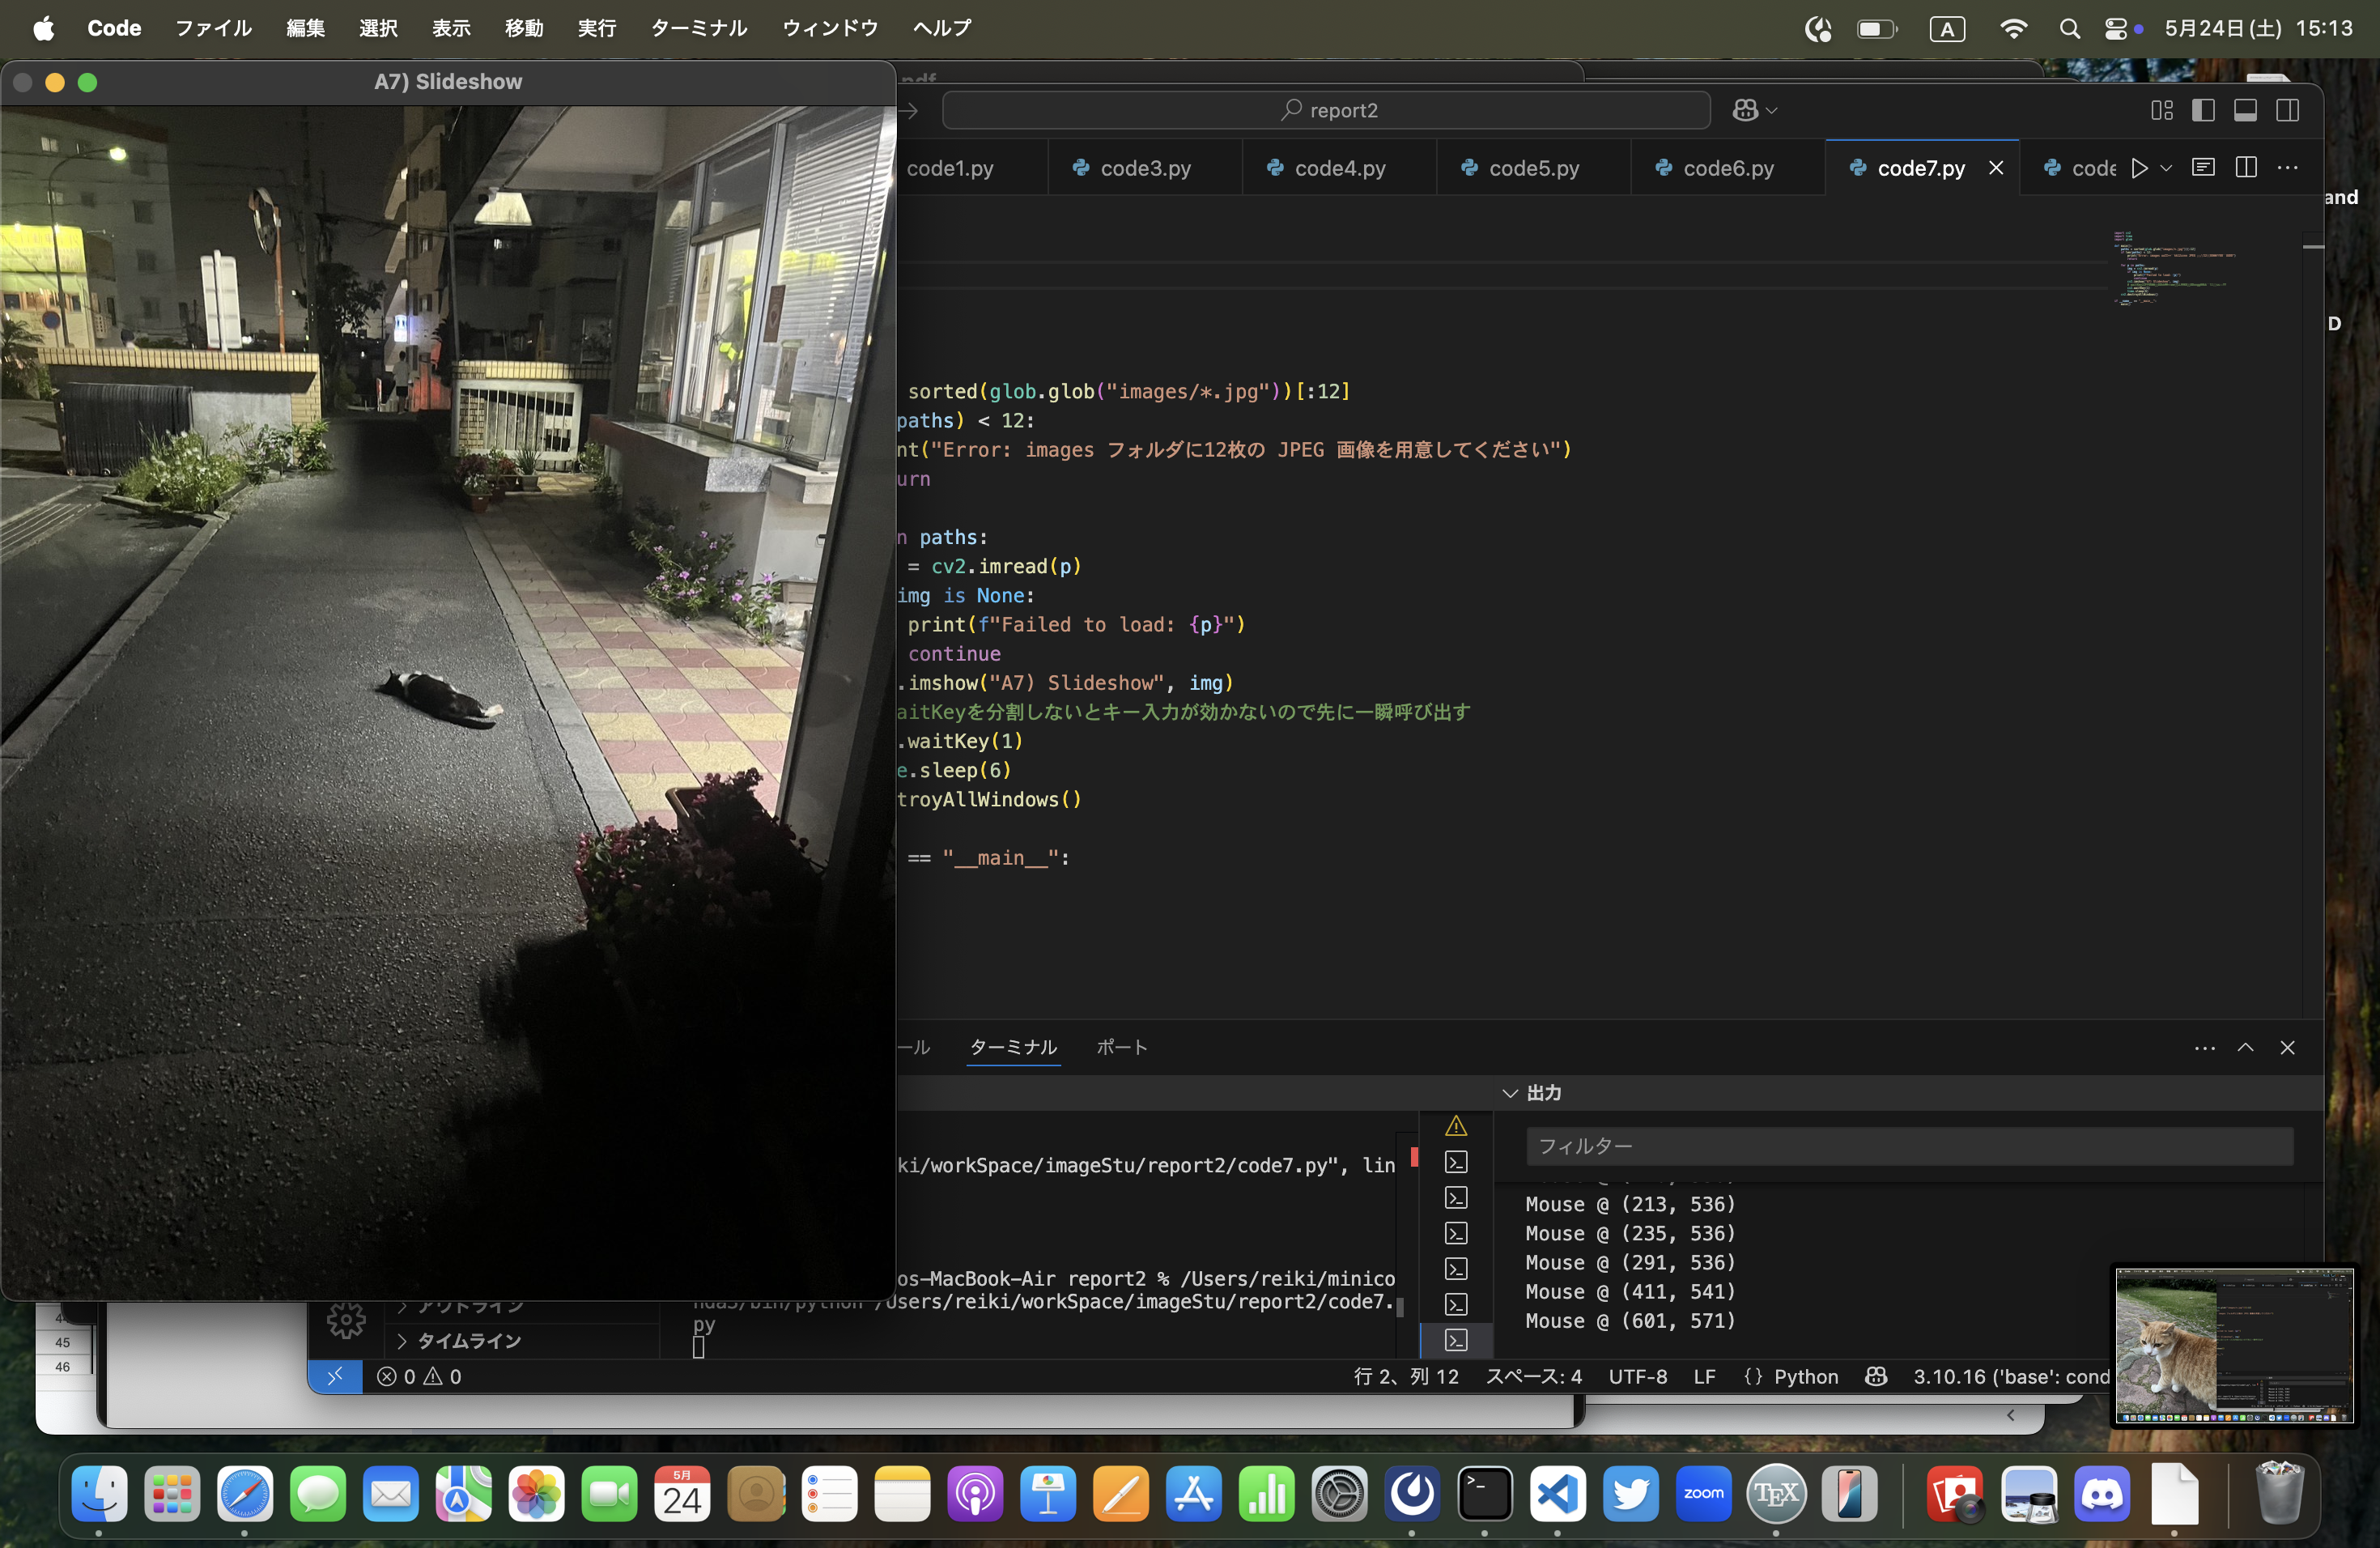
\includegraphics[width=0.8\textwidth]{code7-picture2.png}
  \caption{課題A7 実行結果2}
\end{figure}

\subsection{A8) 12枚の画像を4×3に並べて同時表示}
\lstinputlisting[caption={課題A8: 12枚表示}, label={lst:code8}]{code8.py}
\begin{figure}[H]
  \centering
  \includegraphics[width=0.8\textwidth]{code8-picture.png}
  \caption{課題A8 実行結果}
\end{figure}

\subsection{A9) 任意の1つをクリックで消去}
\lstinputlisting[caption={課題A9: 12枚表示、クリックで削除}, label={lst:code9}]{code9.py}
\begin{figure}[H]
  \centering
  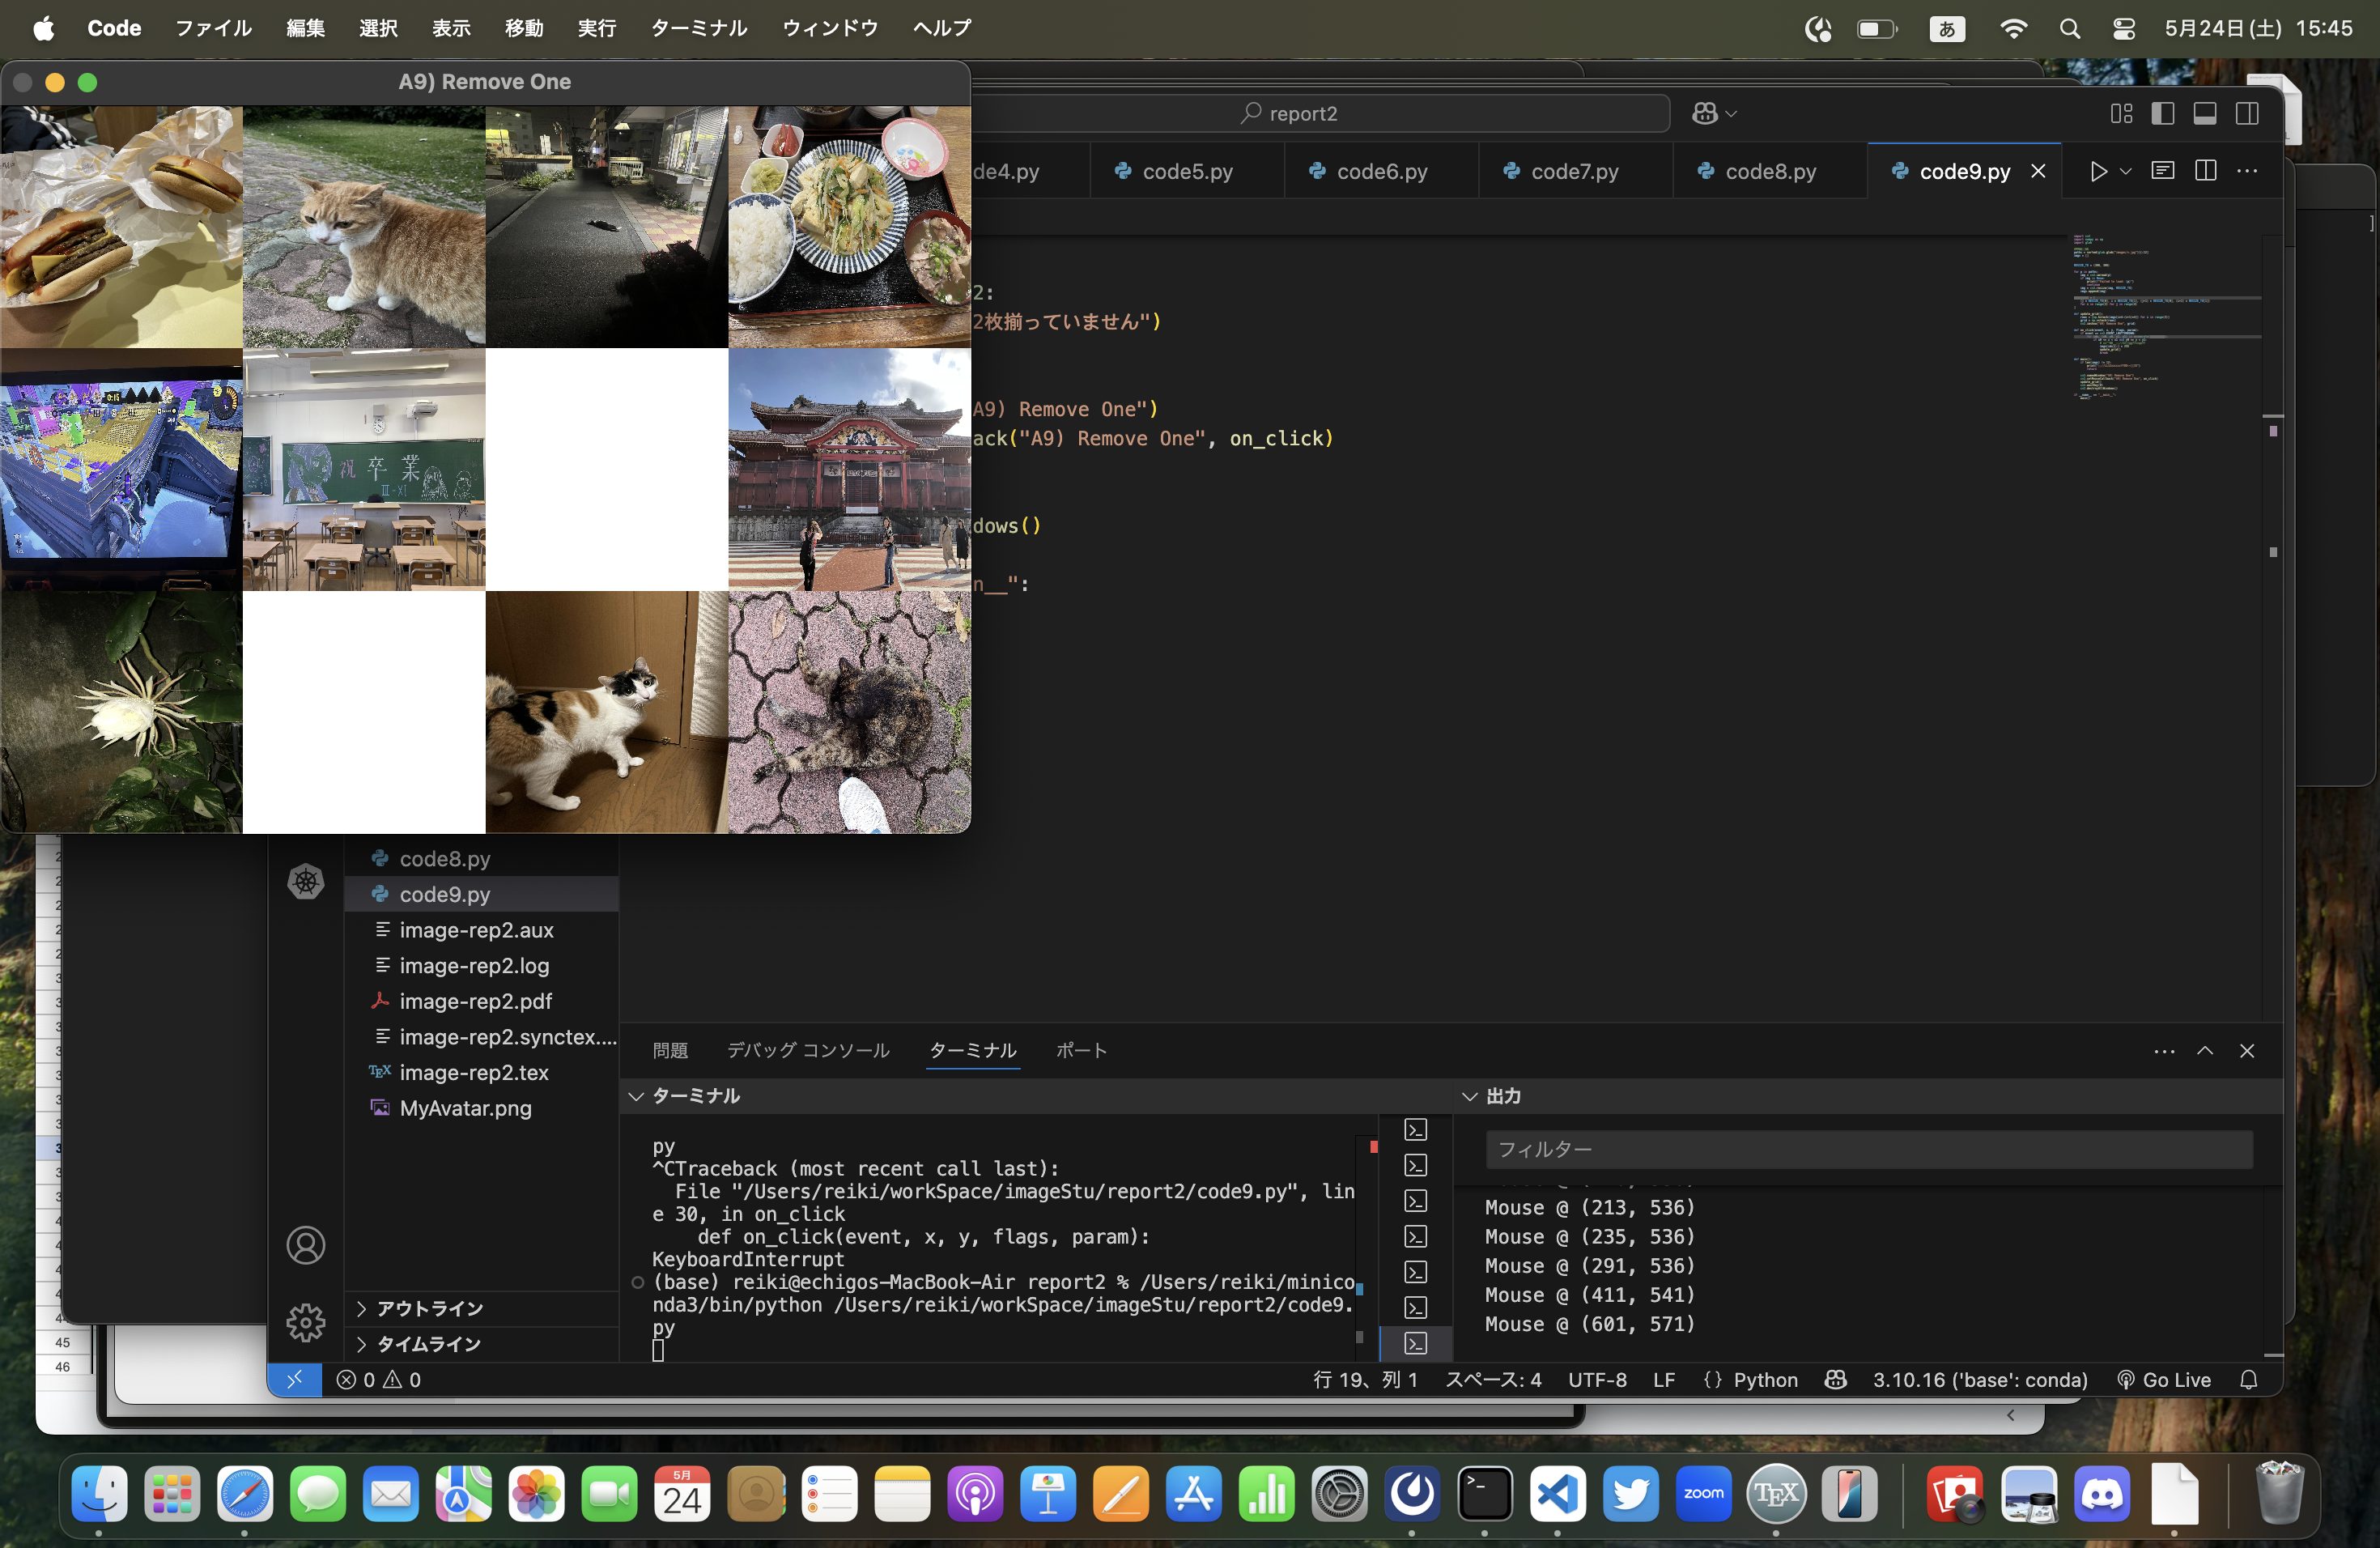
\includegraphics[width=0.8\textwidth]{code9-picture.png}
  \caption{課題A9 実行結果}
\end{figure}

\subsection{A10) 任意の2つをクリックで入れ替え}
\lstinputlisting[caption={課題A10: 12枚表示、クリックで入れ替え}, label={lst:code10}]{code10.py}
\begin{figure}[H]
  \centering
  \includegraphics[width=0.8\textwidth]{code10-picture1.png}
  \caption{課題A10 実行結果1}
\end{figure}
\begin{figure}[H]
  \centering
  \includegraphics[width=0.8\textwidth]{code10-picture2.png}
  \caption{課題A10 実行結果2}
\end{figure}

\end{document}
